\documentclass{style/llncs}

\usepackage{amsmath,amsfonts}
\usepackage{color}
\usepackage[usenames,dvipsnames,svgnames,table]{xcolor}
\usepackage[mathscr]{eucal}
\usepackage{thmtools}
\usepackage{graphicx}
\usepackage{caption}

\newcommand{\M}{\mathscr M}
\newcommand{\C}{\mathscr C}
\newcommand{\T}{\mathscr T}
\newcommand{\F}{\mathscr F}
\renewcommand{\P}{\mathscr P}
\newcommand{\K}{\mathscr K}
\newcommand{\X}{\mathscr X}
\newcommand{\B}{\mathbb B}
\newcommand{\D}{\Delta}
\newcommand{\N}{\mathbb N}
\newcommand{\tn}[1]{\textnormal{#1}}
\newcommand{\pair}[1]{\left\langle{#1}\right\rangle}
\newcommand{\concat}{\oplus}
\newcommand{\symb}[1]{\texttt{#1}}
\newcommand{\br}[1]{\overline{#1}}
\newcommand{\s}{S}
\newcommand{\dom}[1]{\mathop{\tn{dom}(#1)}}
\newcommand{\range}[1]{\mathop{\tn{range}(#1)}}

\newtheorem{conj}{Conjecture}

\let\doendproof\endproof
\renewcommand\endproof{~\hfill\qed\doendproof}

\newcommand{\p}{\,\text{.}}

\newcommand{\tuple}[1]{\left\langle{#1}\right\rangle}

\newcommand{\hide}[1]{}
\newcommand{\old}[1]{}

\newcommand{\sdr}[1]{\textcolor{blue}{\small #1\textsuperscript{[Steven]} }}
\newcommand{\pb}[1]{\textcolor{OliveGreen}{\small #1 \textsuperscript{[Peter]} }}

\newcommand{\argmin}{\mathop{\arg\min}}

% --- DELETE BEFORE SUBMISSIONS ---
\pagestyle{headings} 

\title{Two Problems for Sophistication}

\author{Peter Bloem and Steven de Rooij}

\institute{
  System and Network Engineering Group, \\University of Amsterdam, the Netherlands\\
  \email{uva@peterbloem.nl, steven.de.rooij@gmail.com}
}

\begin{document} 
\maketitle

\begin{abstract}
Kolmogorov complexity measures the amount of information in data, but does not distinguish structure from noise. Kolmogorov's definition of the \emph{structure function} was the first attempt to measure only the structural information in data, by measuring the complexity of an objectively best model under two-part coding. Since then, many variations of this idea have been proposed, for which we use \emph{sophistication} as an umbrella term. We describe two fundamental problems with all existing proposals, showing each  to be \emph{unsound}. Consequently, we put forward the view that the problem is fundamental: it may be impossible to objectively quantify the sophistication.
\end{abstract}

\section{Introduction}\enlargethispage{4ex}
Komogorov complexity gives us a sound definition of the amount of information contained in a binary string. It is, however, not what most people would consider complexity. For example, a sequence of a million coin flips will almost certainly have maximal Kolmogorov complexity, even though there is nothing complex about flipping a lot of coins---it's just a lot of work. Many scholars have defined alternative complexity measures in the spirit of Kolmogorov complexity, aimed at quantifying not \emph{all} information in a binary string, but only the \emph{meaningful} information in the data: its \emph{sophistication}. In this paper, we investigate two serious problems with sophistication measures, and show why they are unsatisfactory. We believe that the problems are fundamental, and provide arguments why attempts to define sophistication must fail.

The Kolmogorov complexity $C(x)$ of a binary string $x$, is (roughly) the length of the shortest computer program that will output $x$. This length depends on which programming language is used, but, as shown by a central result known as the Invariance Theorem\cite[Section~2.1]{li1993introduction}, the language affects the value only by a constant, independent of $x$. This means that for sufficiently complex objects, the choice of programming language becomes irrelevant and Kolmogorov complexity becomes an \emph{objective} measure of the complexity of binary strings, a \emph{property} of the data. A definition of sophistication $S(x)$ in the spirit of Kolmogorov complexity should have similar robustness guarantees:

\begin{enumerate}
\item $S(x)$ should count the bits required for an effective description of the structural properties of a binary string.
\item An analogue of invariance should hold: there must be strict limits on how much sophistication can be affected by a change in programming language.
\item There should be no constant $c$ such that $S(x)\le c$ for every input $x$. If sophistication is bounded, then knowing its value under one programming language provides no constraints on its value under another language (except that it's also bounded). Moreover, a bounded sophistication would be at odds with the intuition that there is no limit to the amount of structure that a binary string can exhibit.
\item Similarly, there should be no constant $c$ such that $C(x)-S(x)\le c$ for all $x$, because then sophistication would be equivalent to Kolmogorov complexity. 
\end{enumerate}
There have been many related proposals for such a measure, that are all based on a \emph{two-part code}: rather than encoding $x$ by means of a single computer program, we encode a \emph{model} for $x$ in the first part of the code, that is interpreted as a representation of $x$'s structural properties. The model does not fully specify $x$, but when combined with the second part of the code, which specifies the noise, the original string becomes fully determined. Thus, the model can be interpreted as a function mapping the noise to the original object.

For any string $x$, there may be many different two-part representations. The total codelength can never be less than the Kolmogorov complexity, but it can come close. The balance between the two parts may vary; Figure~\ref{fig:diagram} provides an illustration. The various proposals then define sophistication in terms of the length of the structure part of this two-part code for one of the representations that (almost) achieves the Kolmogorov complexity. However, for most of these definitions, we can prove that they fail one or more of the conditions above. Vereshchagin and Vit\'anyi's definition \cite{vitanyi2004meaningful} is the one exception that we cannot \emph{prove} to conflict with our requirements, but we show that their method only assigns substantial sophistication to strings that require an enormous amount of processing to construct.

\begin{figure*}[tb]
  \hspace{-2.8em}
  \begin{minipage}{0.55\textwidth}
     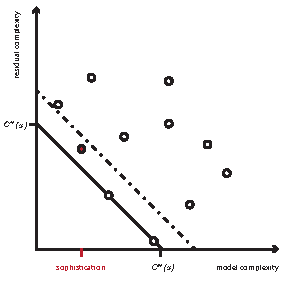
\includegraphics[width=\textwidth]{./img/sophistication.pdf}
  \end{minipage}
  \begin{minipage}{0.55\textwidth}
     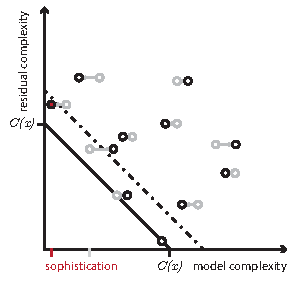
\includegraphics[width=\textwidth]{./img/sophistication-jump.pdf}
  \end{minipage}
  \caption{\small (left) Two-part representations of $x$ by the two components of their codelength. The Kolmogorov complexity $C^\M(x)$, appearing as a black diagonal, provides a lower bound on the total codelength. We consider only representations that are close to this optimum, with the threshold represented by a dashed line. The size of the smallest model below the threshold is the sophistication of the data. (right) The same image, after a constant perturbation in the model complexity caused by a change in numbering.}
  \label{fig:diagram}
\end{figure*}

A valid definition of $S$ must contend with two important issues. First, the details of the way the model is encoded are important. There are two technically distinct approaches; in one of these one has to deal with the so-called ``nickname problem'' that strangely remains unresolved in several publications. These definitions yield a sophistication that is highly dependent on the chosen programming language, unless special care is taken, as discussed in Section~\ref{section:indices}.

The second issue is that of striking the right balance between underfitting and overfitting, which we consider in Section~\ref{section:balance}. Overfitting is a common problem in the statistical literature, that refers to the tendency of model selection to choose a complex model that provides a very good fit to the observed data, but does not generalise well to unseen data. In the case of sophistication, overfitting occurs if the model that determines the sophistication contains much or even all of the noise. This is a real danger, because the models are encoded so efficiently. In statistics, overfitting is often addressed by penalising complex models. In sophistication, however, such penalties tend to break the balance between structural information and noise, and lead to the opposite problem: underfitting.

Underfitting occurs when the selected model is simple, but fails to represent some of the structure present in the data. This is also a problem for sophistication because the considered models are so powerful. In particular, in any programming language, there are programs that implement an interpreter for \emph{another} language. Such \emph{universal models} are \emph{simple} in the language of sophistication, since they can be described with a relatively small number of bits, yet are able to represent the data within a codelength a constant away from the Kolmogorov complexity. Such a two-part representation essentially encodes all information as noise. If complex models are penalized, then the problem becomes to make sure that universal models are not \emph{always} preferred for complex data. The usual workaround is to restrict the set of allowed models to exclude the universal ones. For example, the model class may be restricted to the set of all total recursive functions. While this excludes universal models, it is questionable whether it adequately solves the problem of underfitting in general.

Finally, in the discussion in Section~\ref{section:conclusion} we argue that while two-part coding can yield useful insights into the structure of the data and allows us to identify some models as poor representations, it is probably not possible to uniquely separate structure from noise and identify a \emph{single} model as ``best'': in general many models, of vastly different complexities, may be reasonable representations. Rather than doggedly trying to ``fix'' this property of algorithmic statistics, we propose embracing the idea that the data allows for multiple equivalent interpretations of which information is structured, and which is random, and that there is no such thing as sophistication.

\subsection{Related work}
The idea of separating structure from noise originated with Kolmogorov's \emph{structure function} \cite{cover1985kolmogorov}. In this theory, the data $x$ is described as finite set $A$ that contains $x$, together with the index of $x$ in $A$. The complexity of the set determines the sophistication. This approach was discussed more extensively, and generalised in \cite{vereshchagin2004kolmogorov,gacs2001algorithmic}. 

Koppel \cite{koppelSoph1988,koppel1991almost} also built on the structure function work to define a measure of the meaningful information in a binary string, coining \emph{sophistication}, the name we adopt in this paper. 

In 1996 Gell-Mann and Lloyd introduced \emph{effective complexity} \cite{gellmann1996information}. Working from the perspective of statistical mechanics, they arrived (independently, it seems) at a notion that fits the mold of sophistication.

Adriaans' \emph{Facticity}, introduced in 2012\cite{adriaans2012facticity}, relaxes the model class to include all partial recursive functions. Adriaans also identifies the nickname problem discussed in Section~\ref{section:indices}.

Other authors have pointed out problems with sophistication. Antunes et al. \cite{antunes2009sophistication} note that the constant cutoff used by Koppel is a source of instability, a result in the spirit of this paper. They propose a different definition called \emph{coarse sophistication}. This version behaves very differently from regular sophistication, and is closer to computational depth. Vereshchagin \cite{vereshchagin2013algorithmic} also points out that the Kolmogorov minimal sufficient statistic is not always well-defined and suggests requiring that the finite set model should described using a \emph{total} function rather than any computable function. This yields a more robust sophistication that is nonetheless still susceptible to the issues discussed in this paper.
\section{Preliminaries}
Let $\B = \{0,1\}^*$. We deal with partial computable functions $\phi: \B \to \B$, which we will also call \emph{models}. A function is called \emph{prefix} if its domain, $\dom{f} = \{y : f(y) \neq \infty\}$ is a prefix free set, i.e. no string in $\dom{f}$ is a prefix of another. A function $f$ is \emph{total} if $\dom{f} = \B$.

A \emph{numbering} is an enumeration of of the partial computable functions, denoted as $\psi_1, \psi_2, \ldots$ or simply $\psi$. We fix one canonical effective numbering $\phi$. We call a numbering $\psi$ \emph{acceptable} if there exist total, computable functions $a, b: \N \to \N$ with $\forall: i$, $\phi_i = \psi_{b(i)}$ and  $\psi_i = \phi_{a(i)}$.

A \emph{model class} is a set of model indices. We distinguish four important model classes: 
\begin{enumerate}
\item $\C=\N$, the indices of all partial computable functions
\item $\T=\{i:\tn{$\phi_i$ is total}\}$. Note that $\T$ is not computably enumerable.
\item $\K$ is an enumerable set such that $\{\phi_i:i\in\K\}$ is the set of all partial computable prefix functions
\item $\F$ is an enumerable set such that $\{\phi_i:i\in\F\}$ contains a uniform code for every finite set. A uniform code for a finite set $S$ is a total computable surjective function $f:\{0,1\}^{\lceil\log|S|\rceil}\to S$.
\end{enumerate}
We sometimes need to map binary strings to a prefix-free set. We denote by $\br{x}$ the prefix-encoded representation for $x$. We require that the mapping satisfies $|\br{x}| = |x|+O(\log(|x|)$ (see eg. \cite[Section~1.4]{li1993introduction}). To simplify notation, we will sometimes conflate natural numbers and binary strings, implicitly using the ordering $(0, \epsilon)$, $(1, 0)$, $(2, 1)$, $(3, 00)$, $(4, 01)$, \ldots

Now define the Kolmogorov complexity of a binary string $x$, with respect to a model class $\M$ and a numbering $\psi$, as follows:
\[
C^{\M,\psi}(x)=\min\{\bar\imath y:\psi_i(y)=x,i\in\M\}.
\]
The model class $\C$ gives us the plain Kolmogorov complexity and $\K$ gives us the prefix-free Kolmogorov complexity. For $\C$ and $\K$, the complexity is invariant under a change of numbering, which may therefore be omitted from the superscript.

A pair $(i,y)$ is a \emph{representation} for $x$ if $\phi_i(y)=x$.

\section{Inefficient indices}
\label{section:indices}
In some works, the definition of sophistication is obtained by opening up the definition of Kolmogorov complexity, and measuring the length of the index part of that two-part code. We call such a sophistication \emph{index sophistication}. Examples are Koppel and Atlan's works \cite{koppelSoph1988,koppel1991almost},  and several of its variants \cite{antunes2009sophistication,antunes2013sophistication}. 

In these works, no constraints are placed on the numbering. This makes these approaches vulnerable to the so-called \emph{nickname problem}: the number of bits required to specify a model becomes very dependent on the numbering. This problem is severe: \emph{any} index sophistication without requirements on the numbering is either bounded, or nowhere near invariant:

\begin{lemma}
Let $s^\psi$ denote any index sophistication with respect to numbering $\psi$.
There are acceptable numberings $\psi$ and $\xi$ such that for all $x$
\[|s^\psi(x) - s^\xi(x)|\geq \tfrac{1}{2}\min\{s^\psi(x),s^\xi(x)\}\p\]
\end{lemma}

To prove this, we simply use extremely inefficient numberings:

\begin{proof}
Let $s_i$ be the binary string consisting of $2^{i}$ zeroes followed by a one.

Define $\psi$ and $\xi$ by
\[
\psi_j(x) = \begin{cases}
	\phi_i(x) \;\text{if}\; j = s_{2i}\\
	\infty\;\text{otherwise}
\end{cases}\,\,\,
\xi_j(x) = 
\begin{cases}
	\phi_i(x) \;\text{if}\; j = s_{2i+1} \\
	\infty \;\text{otherwise}\p
\end{cases}
\]
Choose any $x$ and assume w.l.o.g. that $s^\psi(x)\le s^\xi(x)$. By construction of $\psi$ and $\xi$ we have $2s_\psi(x)  \leq s_\xi(x)$ from which the result follows.
\end{proof}
Thus, even though the Kolmogorov complexity changes by only a constant number of bits under a switch to a different numbering, the plain length of the index in a given acceptable numbering is a very poor indicator of model complexity.

In order to obtain a reasonable and robust measure of model complexity, we define the Kolmogorov complexity of functions as in \cite{grunwald2004shannon,vitanyi2004meaningful} by $C^{\M,\psi}(f) = \min\{C^{\M,\psi}(i):\phi_i=f\}$.
Lemma~\ref{lemma:invariance} in the appendix shows that this definition is invariant: the Kolmogorov complexity is an objective property of a function.

There are two ways to use this notion of model complexity for more robust attempts to define sophistication. Confusingly, both approaches are used in the literature.
First, we can measure the complexity of the \emph{model} using $C^{\M,\psi}(\phi_i)$, which is then the first part of a two-part code describing the data. This approach is used in  \cite{cover1985kolmogorov,gacs2001algorithmic,vitanyi2004meaningful,gellmann1996information} and in most of the present paper.

Second, we can stick to using the length of the index as the measure of sophistication, but impose the additional constraint that an efficient acceptable numbering is used. This is the approach taken by Adriaans \cite{adriaans2012facticity}.  Before switching to the other approach we construct such an efficient index.

We call a numbering $\psi$ \emph{faithful} if for all $i$ there is a $j$ such that $\psi_i=\psi_j$ and $|j|\le C^{\C}(\psi_j)+c$, for some constant $c$. This definition is a refinement of \cite[Definition~10]{adriaans2012facticity}. We prove in the appendix that there actually do exist faithful, acceptable numberings (Lemma~\ref{lemma:faithful-numberings}). However even choosing a faithful index is not quite enough. The Kolmogorov complexity uses representations of the form $\bar\imath y$, where the bar denotes some straightforward prefix encoding to delimit the model description $i$ from its input $y$. If we define a second prefix encoding $\tilde{\imath}$, with $|\bar\imath|-|\tilde\imath|$ unbounded, we can define a second representation $\bar u \tilde \imath y$, at a constant overhead $|\br{u}|$, and gain more than $|\br{u}|$ for sufficiently complex strings. As shown in Lemma~\ref{lemma:prefix-inefficiency} in the appendix, this results in a bounded sophistication. 
This is in fact an issue with \cite{adriaans2012facticity}. Moreover, we conjecture that \emph{no} computable prefix function $\bar\cdot$ is sufficiently efficient to avoid this.

Because of these issues, rather than index sophistication we will use the following definition of sophistication in the remainder of this article. It is parameterised by a model class, a numbering, and a slack parameter $c$ that determines the maximal allowed slack between the two-part code length using a representation and the Kolmogorov complexity.
\[
S^{\M,\psi,c}(x)=\min\left\{C^\K(\phi_i):i\in\M,C^{\{i\},\psi}(x)\le C^{\M,\psi}(x)+c\right\}.
\]

\section{Balancing under- and overfitting}
\label{section:balance}

In the previous section, we saw the first glimpse of the delicate balance between the two code components in sophistication. If the description of the model $m$ is less efficient than $C^\K(m)$ by anything more than a constant, the sophistication becomes bounded. We will investigate this balance, starting with the sophistication $S^{\K,\psi,c}$. In this setting, we know that, on the one hand, there always exist candidate models---those models $i$ with $i \in \K$ and $C^{i}(x) \leq C^\K(x) + c$---for which al information except a constant amount is stored in the data, and on the other hand, there are also candidate representations for which all information is stored in the model. This tells us that $S^\K$ is \emph{balanced}: there is no inefficiency in the representation forcing information in or out of the model.
The flip side of having a balanced sophistication is that it becomes easy to show invariance. We will show that there are numberings for which the universal models always determine the $S^\K$ and numberings for which the singletons always determine $S^\K$. The following lemma is based on the idea that, given a subset $\M'$ of the model class, we can choose the numbering so that representations use a model in $\M'$ perform an arbitrary constant better than all other models, so that a model in $\M'$ always ends up determining the sophistication.
\begin{restatable}{lemma}{coolone}
\label{lemma:thecoolone}
  Let $\M$ be any model class, let $\X$ be any set of binary strings and let $D:\B\to\N$ be a computable decoding function with a prefix-free domain that maps function descriptions to their indices in $\phi$, i.e. if $m=\phi_{D(p)}$ then $p$ is a $D$-description of $m$. Let $\M'=\{\phi_i:i\in\tn{range}(D)\}$. Further assume there is a constant $c$ such that:\\
\-\hspace{1cm}(1) $\forall_{m\in\M'}:\min\{|p|:\phi_{D(p)}=m\}\le C^{\K,\phi}(m)+c$\\
\-\hspace{1cm}(2) $\forall_{x\in\X}:C^{\M',\phi}(x)-C^{\M,\phi}(x)\le c$.\\
Then there is an enumeration $\psi$ of the partial recursive functions such that $S^{\M,\psi}(x) = |\br{0}|+S^{\M',\phi}(x)$ for all $x\in\X$.
\end{restatable}
This means that for model classes with a universal model, there is a numbering such that sophistication is bounded:
\begin{restatable}[underfitting]{lemma}{underfitting}
Let $\M$ be a model class containing a universal model $\phi_u$, with the property that $\exists c \forall i \in \M : C^{\{u\}}(x) \leq C^{\{i\}}(x) + c \p$. Then, there exist numberings such that $\s^\M$ is bounded.
\end{restatable}
\noindent For other numberings, the singletons determine the sophistication, making it equal to the complexity:
\begin{restatable}[Overfitting]{lemma}{overfitting}
Let $\M \subseteq \K$ be a model class where for every $x\in\X$ there is a singleton model $i\in\M$ with $\phi_i(\epsilon)=x$. Then there is a numbering $\psi$, and a constant $c$, such that for all $x\in\X$ we have $C^\M(x)-S^{\M,\psi}(x)\leq c$.\label{lemma:overfitting}
\end{restatable}
\noindent Thus, in this balanced sophistication, there is no invariance: all information can be seen as structure, or as noise, depending on the numbering. To avoid these issues, existing proposals upset the balance to exclude or penalize at least the singleton models and the universal models.
 
\subsection{Overfitting}

The existing proposals that can overfit are the minimal sufficient statistic in the structure function \cite{cover1985kolmogorov}, the sophistication as defined in \cite{mota2013sophistication}, the minimal sufficient algorithmic statistic \cite{gacs2001algorithmic} and Vereshchagin's strongly sufficient statistic \cite{vereshchagin2013algorithmic}. It is widely recognized that singleton models are always candidates in these settings, but not, it seems, that they may be the only candidates for any string, as Lemma~\ref{lemma:overfitting} shows. 

It may be argued that the slack parameter $c$ in the sophistication, that determines the allowed gap between a candidate representation and the complexity, should be allowed to depend on the numbering, but this dependence has not been mentioned in the literature and there is no clear way to determine how this constant should be determined on the basis of a given numbering. 

In traditional statistics, overfitting is often addressed by imposing a penalty on complex models. As we have seen, a strong penalty, such as the one imposed by an inefficient prefix encoding of the model, will immediately cause underfitting. A more subtle approach is to use $\C$ as a model class rather than $\K$, thus allowing representations that are not self-delimiting. The gap between self-delimiting and non self-delimiting descriptions grows without bound 
\cite[Section~4.5.5]{vitanyi2004meaningful}, so that for sufficiently complex inputs all information will have to be placed in the noise part of the code, eliminating the singletons as viable candidates. This approach is taken by Vit\'anyi \cite{vitanyi2004meaningful} and by Adriaans \cite{adriaans2012facticity}. Such measures thus help reduce the overfitting problem, but they only increase the tendency to underfit. We also pay the price that the models can no longer be equated with probability measures, removing the link to traditional statistics and probability theory.

\subsection{Underfitting}

As mentioned in the related work, underfitting is a widely acknowledged problem for sophistication, and most proposals avoid it by limiting the class of allowed models, to exclude universal models. The following theorem shows that this does indeed yield an unbounded sophistication.

\begin{restatable}{theorem}{dogfood}
There are infinitely many $x$ with $\s^{\F,\phi,c}(x) \geq C^{\K}(x)/5$, and also infinitely many $x$ with $\s^{\T,\phi,c}(x) \geq C^{\K}(x)/6$.
\end{restatable} 

Thus, there are no longer any numberings for which sophistication is bounded, so the underfitting problem is at least partly solved. However, as we show below, the resulting sophistication is not an intuitive measure of the amount of structure in the data. Moreover, we push the balance back in the direction of overfitting, which is only exacerbated by this change. Only one model class eliminates both the singletons and the universal model: $\T$. The only proposal that uses an efficient model representation \emph{and} excludes the universal models \emph{and} excludes the singletons is Vereshchagin and Vit\'anyi's \cite{vitanyi2004meaningful}. While this invalidates straightforward proofs of boundedness, there is no suggestion that $S^{\T, \phi, c}(x)$ is actually invariant.

While under $S^{\T, \phi, c}(x)$ there are strings with high sophistication, these may not conform to the original intuition that motivated sophistication. To show this, we need the concept of depth:

\begin{definition}[Depth\cite{bennett1988logical,antunes2006computational}]\belowdisplayskip=-12pt
Let $U$ be some universal Turing machine, so that $U(\bar\imath y) = \phi_i(y)$. Let $U^t$ be a simulation of this machine, which is allowed to run for at most $t$ steps, and returns $0$ if it has not yet finished at that point. Let $C^\M_t(x) = \min\{|\bar\imath y| : U^t(\bar\imath y) = x, \phi_i \in \M\}$. The \emph{$c$-depth} is $d^{\M,c}(x) = \min \left\{t : C^\M_t(x) - C^\M(x) \leq c \right\}$.
\end{definition}
Deep strings are those that can only be optimally compressed with a great investment of time. We note that it is exceedingly unlikely that a deep string is sampled from a shallow distribution \cite{bloem2014safe,bennett1988logical}.
 
\begin{restatable}{theorem}{depth}
Let $A(n)$ be the single-argument Ackermann function and $c$ some arbitrary constant. There are numberings such that for strings with depth $d^{\C,c}(x) \leq A(C^\C(x))$ the sophistication $\s^{\T, \psi, c}$ is bounded. The same is true for $\s^{\F}$ .
\end{restatable}
\noindent This shows that while high-sophistication strings do exist, they do not behave as expected. Consider a string that is typical for a shallow model, say some elaborate Markov chain. Under $\s^{\T,\psi,c}$, no matter how long an effective description of the Markov chain would have to be, the sophistication is bounded. Any structure that is simple enough to be exploited within the time bound of the Ackermann function (or some other fast-growing, simply stated bound) will be counted as noise. Only structure that is so deep that if we used it to compress $x$ we could never hope to decompress it within the lifetime of the universe, would count towards sophistication. 
This clearly contradicts the motivating principle of sophistication, which is to capture the number of bits required to express \emph{all} regularity in the data, not just the regularity that is difficult to describe. 
In this setting, a string high-sophistication not only has a lot of structure, but it also has the property that it can be compressed far better with partial functions than with total. That is, it is non-typical for the model class $\T$. This suggests that the `non-stochastic' property of strings with high sophistication \cite{shen1983concept,vereshchagin2004kolmogorov} says more about depth and totality than it does about structure and noise.

The relation between sophistication, depth and absolutely non-stochastic strings was also investigated in \cite{antunes2013sophistication}.

\section{Discussion and conclusion}
\label{section:conclusion} 

We have criticized existing measures of the sophistication of a binary string. Our results show that there are technical problems with all of them. But that does not in itself mean that it should be impossible to come up with a sound measure. The intuition throughout the literature, starting with the structure function, appears to be that the crucial property is whether a string is typical for a model. If so, another random choice from that mode selects a string with the same structure: a string of the same `type'.

This idea is bold, but not necessarily unreasonable. Nevertheless, in this section we offer the opinion that such a clean-cut separation \emph{cannot} be made to work. We provide two arguments to support this belief.

For the first argument, we take a generative perspective. We can generate data from a model in $\phi_i, i \in \K$ by feeding it random bits until it produces an output. We will call the resulting probability distribution $p_i(x) = \sum_{y:\phi_i(y) = x} 2^{-|y|}$. In this scenario, a sophistication could be called \emph{consistent} if, for data of sufficiently high complexity, it accurately reflects the complexity of that distribution from which it originated. Suppose that the data issampled from  universal distribution: let $\phi_u(\bar\imath y)=\phi_i(y)$ and sample from $p_u$ as described above. Then the initial random bits will determine the prefix encoded index $\bar\imath$ of the function $\phi_i$ that $\phi_u$ will subsequently emulate, and the remaining bits are used as inputs to $\phi_i$. We now ask, what should be the sophistication of the resulting data?

Certainly, if we have to judge based only on the data, we cannot exclude the possibility that the data was sampled from $p_u$: after all, it was.  On the other hand, neither can we exclude the possibility that it came from $p_i$, as again, it did! It seems unjustified to assume that, based on only the data, all but one model can always be disqualified.

Consider the following metaphor. We are given a bitstring which can be read as a bitmap image of the painting \emph{Impression of a Sunrise}. There are many good models for this string, ranging from very generic to very specific. The theory behind sophistication suggests that we can choose one of these as the objective, intrinsic model of the data. Different models say different things: the universal model says that it is `some finite object'. A more specific model might say that it is `an image'. Even more specific would be a painting, a Monet, or specifically the painting Impression of a Sunrise. A sound measure of Sophistication should be able to select one of these models as the proper representation of structure in the data, and disqualify the others as either over- or underfitting. But how should we be able to say that the data is intrinsically more of a painting than an image? More of a Monet than a painting? Intuitively, such distinctions require further assumptions, or a second sample from the same distribution.

The second reason we believe sophistication will elude definition is more technical. Given an input $x$ and some model class, say $\C$, consider the set of all possible two-part representations of $x$. Now, when the numbering of partial computable functions is changed, the codelength of the model part of all these representations will change. This is illustrated in the right graph in Figure~\ref{fig:diagram}. However, the Invariance Theorem expresses that this change is limited by a constant term that does not depend on $x$. So for sufficiently large $x$, the horizontal shift of all the representations will be relatively small. However, even this small shift can push some representations out of the acceptable region (indicated by the dashed line), and pull others in. This may lead to a different representation determining the sophistication, one whose \emph{total} codelength is close to what it was before, but whose \emph{model} codelength can be anywhere between $0$ and $C^\C(x)$. If such jumps can occur, the sophistication is not invariant. And while we cannot \emph{prove} in general that such jumps can always occur, there seems to be no reason to believe that they don't.

For this reason, we take a skeptical view of sophistication. Note that part of the theory is fine: there is nothing wrong with evaluating models for the data by comparing their two-part code lengths. In fact, the randomness deficiency $\delta(\phi_i,x)=-\log p_i(x)-C^\K(x\mid i)$ of a model $\phi_i$ has a direct statistical interpretation as a measure of counterevidence against the hypothesis that it generated the data---if $p_i$ truly generated the data, then the probability that the randomness deficiency is more than $k$ bits is less than $2^{-k}$ \cite{bloem2014safe}[Lemma~6]. In the Monet example above, this will allow us to disqualify the model expressing that the data is actually, say, a recording of Jazz music.

But fundamental problems arise as soon as hard cut-offs are introduced. In our opinion, a lot of measures taken in the literature to address problems with sophistication, such as restricting the model class or introducing model penalties, complicate the method and make problems harder to analyse, without actually addressing the fundamental issue. This is dangerous: if such ad-hoc fixes result in a theory that is hard to prove either wrong or right, it creates an artificial dead end for a valuable area of research. When hard cut-offs are avoided, on the other hand, all such measures are suddenly no longer necessary. What remains is a simple and elegant theory that can be used to sift through all possible models, disproving most while retaining a select number of interesting candidates for our further consideration.

\subsubsection*{\ackname}

This publication was supported by the Dutch national program COMMIT and by  the Netherlands eScience center.

\bibliographystyle{plain}
\bibliography{facticity}

\appendix

\section{Proofs}

\subsection{Invariance of function complexity}

\begin{lemma}[Invariance of function complexity]
Let $\psi$ and $\eta$ be any two acceptable numberings. There exists a constant $c$ such that $\left| C^{\K,\psi}(f) - C^{\K, \eta}(f)\right | \leq c$ for all $f \in \C$ and $\left| C^{\C,\psi}(f) - C^{\C, \eta}(f)\right | \leq c$ for all $f \in \C$. \label{lemma:invariance}
\end{lemma}
\begin{proof}
Let $g(i)$ be the function such that $\psi_i=\eta_{g(i)}$.
\begin{align*}
C^{\C,\psi}(f) &= \min\left\{ C^{\C,\psi}(i) : \psi_i= f\right\} 
\geq \min\left\{ C^{\C, \eta}(i) : \psi_i= f\right\} - c\\
&= \min\left\{ C^{\C, \eta}(i) : \eta_{g(i)}= f\right\} - c
\geq \min\left\{ C^{\C, \eta}(i) : \eta_i= f\right\} - c' \\
&= C^{\C, \eta}(f).
\end{align*}
The opposite inequality can be achieved by reversing $\psi$ and $\eta$. The same proof holds with model class $\K$.
\end{proof}
This lemma shows that the complexity of a function does not depend on the choice of
enumeration by more than a constant term.


\begin{restatable}{lemma}{faithful}\label{lemma:faithful-numberings}
  There are faithful acceptable numberings.
\end{restatable}

\begin{proof}
Let $d \in \N$ be an index such that $\phi_d(y)=\infty$ for all $y$. Define
  \[\psi_q=\begin{cases}
    \phi_{\phi_i(p)}&\tn{if $q$ can be written as $\bar\imath p$ and $\phi_i(p)<\infty$,}\\
    \phi_d&\tn{otherwise.}\end{cases}
  \]
  To show that $\psi$ is faithful, pick any function $f$. Then
\[\begin{split}
C^{\C, \phi}(f)&=\min\{C^{\C, \phi}(i):\phi_i=f\} =\min\{\min\{|\bar a b|:\phi_a(b)=i\}:\phi_i=f\} \\
& =\min\{|\bar a b|:\phi_{\phi_a(b)}=f\}
 =\min\{|\bar a b|:\psi_{\bar a b}=f\}.
\end{split}\]
This shows there is a sufficiently small $\psi$ index.

To show that $\psi$ is acceptable, let $\phi_j$ denote the identity
function. Then a $\phi$-index $i$ can be mapped to a $\psi$-index
using the computable function $r(i)=\bar\jmath i$, so that
$\psi_{r(i)}(y)=\psi_{\bar\jmath i}(y)=\phi_i(y)$. For the reverse,
define $\phi_v(\bar\imath p, y)=\phi_{\phi_i(p)}(y)$. For fixed
$\bar\imath p$, the 
$s^n_m$-theorem \cite{kleene193notation} states that we can compute the $h$
such that $\phi_h(y)=\phi_v(\bar\imath p,y)$. Let $h(\bar\imath p)$
denote this index as a function of the program; further define
$h(q)=d$ if $q$ cannot be expressed as $\bar\imath p$. By
construction $h$ is total and computable. To check that the mapping
returns the correct function, rewrite $\phi_{h(\bar\imath
  p)}(y)=\phi_v(\bar\imath p,y)=\phi_{\phi_i(p)}(y)=\psi_{\bar\imath p}(y)$.
\end{proof}

\subsection{Inefficient indices}
\label{section:appendix-inefficient-indices}

Can we make our prefix encoding $\bar\cdot$ so efficient that no other encoding can undercut it? By definition, $C^{\K}(\phi_i)$ is the smallest effective, self-delimiting description of $\phi_i$. We cannot compute the prefix code from the data, but this is not necessary to define a representation. Let $i^*$ be the shortest self-delimiting program for $\phi_i$, then $i^*y$ is a decodable representation for $x$. If our prefix function is less efficient than $C^\K(m)$ by an unbounded amount, $i^*y$ will always beat $\bar\imath y$ for complex enough data. We conjecture that no computable prefix encoding function can avoid this issue:
\begin{conjecture}
For any partial computable prefix codelength function $L$, the function $\min\{L(i)-C^\K(i):i\ge i_0\}$
is unbounded in $i_0$.
\end{conjecture}
The following lemma shows that even index sophistications using a faithful index are bounded if the prefix encoding is inefficient.

\begin{restatable}{lemma}{ineffprefix}
Assume $\phi$ is faithful and define the index sophistication $s^c(x)=\min\{|\bar\imath|:C^{\{i\}}(x)\le C^{\C}(x)+c\}$.
If $\min\{|\bar\imath|-C^\K(i):i\ge i_0\}$ is an unbounded function of $i_0$, then $s^c$ is bounded.\label{lemma:prefix-inefficiency}
\end{restatable}
If our conjecture is correct, the index sophistication is always bounded for model class $\C$. Any inefficieny in the model description, and a second represention using a universal model with a more efficient model description will win, causing a bounded sophistication.

\begin{proof}
Let $\bar\imath y$ be any two-part representation for the data $x$, i.e. $\phi_i(y)=x$. Then construct an alternative two-part representation $\bar vi^* y$, where $i^*$ is the shortest $\psi_u$-program for $i$ such that $\phi_v(i^* y)=\phi_{\psi_u(i^*)}(y) = \phi_i(y)=x$. We compare the lengths of these two representations. Note that $|i^*|=C^{\K,\phi}(i)$. Therefore,
\[
|\bar\imath y|-|\bar v i^* y| = |\bar\imath|-|\bar v| - |i^*| = |\bar\imath|-|\bar v|-C^{\K}(i).
\]
By assumption there must be an $i_0$ such that the above expression is positive for all $i>i_0$. From this $i_0$ onwards, the second representation (using $v$) will have a shorter codelength, so $\bar\imath p$ cannot achieve the minimum in the definition of the sophistication. Consequently, the sophistication is bounded by $s(x)<|\overline{\imath_0}|$ for all $x$. 
\end{proof}

\subsection{Boosting submodel by manipulating the numbering}

\coolone*

\begin{proof}
We define the numbering $\psi$ as follows:
\[\begin{cases}
\psi_0(p) = 1^r 0 D(p) \\
\psi_{1^r0i}(p) = \phi_i(p) \\
\psi_j(\cdot) = \infty &\text{if $j$ contains no zeroes.}
\end{cases}\]
We will show that under the $\psi$-enumeration, the best representation for $x$ using a model $m\in\M'$ is always better than the best representation using some $m\notin\M'$.

First suppose $m\in\M'$. Then
\begin{align*}
C^{\K,\psi}(m) &=\min\{|\bar\jmath q|:\psi_{\psi_j(q)}=m\}
\leq\min\{|\bar0 q|:\psi_{\psi_0(q)}=m\} \\ 
&=\min\{|\bar0 q|:\psi_{1^r0 D(q)}=m\}  
=\min\{|q|:\phi_{D(q)}=m\} + |\bar 0|\\
&\leq C^{\K,\phi}(m)+c+|\br{0}|,
\end{align*}
where the last inequality uses assumption (1).

Now assume that the best model $m$ for $x$ is not in $\M'$. 
Let $i$ be the index of $m$ with the shortest description, i.e. it achieves the minimum in $C^{\K, \psi}(m)=\min\left\{C^{\K,\psi}(i):\psi_i=m\right\}$.
There are two possibilities. Either $i = 0$, in which case we have $C^{\K,\psi}(m)\ge r$ because $\phi_0$ cannot output zero and all other $\psi$-programs are at least $r$ bits long.

Otherwise, we can bound
\begin{align*}
C^{\K,\psi}(m)&=C^{\K,\psi}(i)=C^{\K,\psi}(1^r0j)\\
&\ge C^{\K,\psi}(j)-c' \ge C^{\K,\phi}(j)+r+1-c'\\
&=C^{\K,\phi}(m)+r+1-c'.
\end{align*}
Now choose $r=c''+\max\left\{C^{\K,\psi}(\phi_0),c'-1\right\}$. Then substitution yields, for both cases, 
$C^{\K,\phi}(m)\ge c''+C^{\K,\psi}(m)$.

Combining the inequalities above, for any model $g\not\in\M'$, there is a model $f\in\M$ such that
\[\begin{split}
C^{\K,\psi}(g)+\min \{|y| : g(y) = x\} &\ge C^{\K,^\phi}(g)+\min\{|y| : g(y) = x\}+c''\\
&\ge C^{\K,\psi}(f)+\min \{|y| : f(y) = x\} -2c+c'' -|\bar0|.
\end{split}\]
By choosing $c''$ sufficiently large, we can ensure that the best representation is in $\M'$ for all $x\in\X$, which completes the proof.
\end{proof}

\subsection{Overfitting}

\overfitting*

\begin{proof}
Let $\phi_i$ be a singleton for $x$ as described. Note that since $\phi_i$ is a prefix function, if $\phi_i$ is defined for input $\epsilon$ then it cannot be defined for any other input. Pick $i,x$ with $\phi_i(\epsilon)=x$. Note that $x$ can be computed from $i$ and a fixed program, so there is a $c$ such that $C^{\K, \phi}(x)\le C^{\K, \phi}(\phi_i)+c$. Vice versa, given any $x$ we can construct an index of $\phi_i$, since $\phi$ is an acceptable numbering. Therefore $|C^{\K,\phi}(\phi_i)-C^{\K, \phi}(x)|\le c$.

We now define a computable function $D$ by $D(\bar\imath y)=j$ where $\psi_j(\epsilon) = \psi_i(y)$.  We will show that the two conditions of Lemma~\ref{lemma:thecoolone} hold for the prefix function $D$.

(1) Let $f$ be any function in the range of $D$, and $x$ its output. Then $\min\{|p|:\psi_{D(p)}=f\}=\min\{|\bar\imath q|:\psi_i(q)=x\}=K(x)\le K(f)+c$. (2) On the one hand $L^{\M',\psi}(x)\le K(f)+|\epsilon|\le K(x)+c$. On the other hand, $L^{\M,\psi}(x)$ is an effective description of $x$, so $K(x)$ is at most a constant larger. Together, these inequalities establish the second condition.

Now, by Lemma~\ref{lemma:thecoolone} there is an enumeration $\phi_1,\phi_2,\ldots$ such that $S^{\M,\phi}(x)=|\bar 0|+S^{\M',\psi}(x)$. We observed that $|K(f)-K(x)|\le c$ for any $f\in\M'$, so $S^{\M',\psi}(x)\ge K(x)+c$. This proves the lemma.
\end{proof}
\subsection{Underfitting}

\underfitting*

\begin{proof}
Let $D$ be a prefix function as in Lemma~\ref{lemma:thecoolone} such that it returns the index of $u$ for the argument $\epsilon$ and $\infty$ for any other argument. That is, $\M' = \{u\}$. This construction satisfies the conditions 1 and 2 from Lemma~\ref{lemma:thecoolone}; invoking it we find that there exists an acceptable numbering for which $\s_\M(x) = \s_{\M'}(x) + c$. Since $\M'$ contains only a single model, $\s_{\M'}$ is constant.
\end{proof}

\subsection{The problem of depth}

We first show that representations using $\T$ can be reduced to representations in $\F$ with a small overhead.

\begin{definition}[Stochastic strings, Definition~1.1 from~\cite{gacs2001algorithmic}]
  Let $\alpha$ and $\beta$ be natural numbers. A finite binary string $x$ is called \emph{$(\alpha,\beta)$-stochastic} if there exists a finite set $S\subseteq\B$ such that 
  \[
  x\in S,~C^\K(S)\le\alpha,~C^\K(x)\ge\log|A|-\beta.
\]
\end{definition}

\begin{restatable}{lemma}{vitanyi}
Let $f$ be a total, computable function, such that for some $d$, $f(d) = x$ and let $k = K(f) + |d|$. Then there exists a finite set $A$ containing $x$ and a constant $c$, such that $K(A) \leq K(f) + K(|d|) + c$ and $\log |A| \leq |d|$.\label{lemma:total-to-sets}
\end{restatable}
\begin{proof}
Let $S = f\left(\{0,1\}^{|d|}\right)$. Since $f$ is total, this set can be explicity computed from a description of $f$ and a description of $|d|$, which tells us that there is a constant $c$ such that $C^\K(A) \leq C^\K(f) + C^\K(|d|) + c$. 

Since $A$ is the image of a set of size $2^{|d|}$ under $f$, we have $\log |A| \leq |d|$.
\end{proof}
\noindent This lemma is a variation on \cite[Lemma~7.2]{vitanyi2004meaningful}. 

We use this to show that sophistications with a restricted model class are not bounded:
\dogfood*
\begin{proof}
In this proof, for convenience we identify the models indexed by $\F$ with the sets that they encode. Thus the two-part code consists of the description of a set $A$, and then an index in this set using $\log|A|$ bits.
For all $i$, let $x_i$ be the smallest binary string that is not $(i/4, i/4)$-stochastic. Since every string is $(\alpha,\alpha)$-stochastic for sufficiently large $\alpha$, this is a sequence of infinitely many distinct binary strings of increasing length. From \cite[Proposition~I.3 (b)]{gacs2001algorithmic} we know that for all sufficiently large $i$ there are strings of length less than $i$ that are not $(i/4, i/4)$-stochastic. Now pick any $i$ that is large enough that (a) $|x_i|<i$ and (b) $C^\K(x_i)/5 < i/4$. By definition of $(\alpha,\beta)$-stochasticity, if a string is not $(i/4,i/4)$-stochastic, then for every finite set $A$ containing $x$, either (a) $\log|A|\ge C^\K(x_i)+i/4\ge 5C^\K(x_i)/4$, or (b) $C^\K(A)>i/4>C^\K(x_i)/5$.
In case (a), any two-part description using $A$ is substantially larger than the Kolmogorov complexity, for large enough $i$, so it does not determine the sophistication. Case (b) provides the required lower bound on the complexity of the model.

Now, take $\T$ as model class and suppose towards contradiction that the sophistication is determined by a total function $f=\phi_j,j\in\T$ with $f(d)=x$ and $C^\K(f)\le i/5$. Then by Lemma~\ref{lemma:total-to-sets}, for some fixed constant $c$ there is a finite set $A$ with $\log|A|\le|d|\le C^\K(x_i)$, so (a) above cannot be the case, and $C^\K(A)\le C^\K(f)+C^\K(|d|)+c\le i/5+C^\K(|d|)+c$, which contradicts (b) for large enough $i$. Therefore such candidates $f$ cannot exist and all candidates must satisfy $C^\K(f)>i/5>C^\K(x_i)/6$.
\end{proof}

Note that we favoured brevity of the proof over the strength of the bounds: the multiplicative constant $1/6$ can be improved with a more detailed treatment.

\depth*
\begin{proof}
Let $U(\bar\imath y)$ be some (non-prefix) universal Turing machine, and let $U^A(\bar\imath y)$ be a simulation of that machine which outputs $0$ if the number of steps taken exceeds $A(|\bar\imath y|)$. Let $u$ be the index of the function $U^A$ in the standard enumeration.

Let $D$ be a prefix function with $D(\epsilon) = u$. We can instantiate Lemma~\ref{lemma:thecoolone} with $D$, $\M' = \{\phi_u\}$ and $X = \{x : d^\C_c(x) \leq A(C(x))\}$. This tells us that there exists a numbering for which $\s^\T(x) = \s^{\M'}(x) + |\bar0| \leq c$ for all $x \in X$.
\end{proof}

\end{document}
